\let\negmedspace\undefined
\let\negthickspace\undefined
\documentclass[journal,12pt,onecolumn]{IEEEtran}
\usepackage{cite}
\usepackage{amsmath,amssymb,amsfonts,amsthm}
\usepackage{algorithmic}
\usepackage{graphicx}
\graphicspath{{./figs/}}
\usepackage{textcomp}
\usepackage{xcolor}
\usepackage{txfonts}
\usepackage{listings}
\usepackage{enumitem}
\usepackage{mathtools}
\usepackage{gensymb}
\usepackage{comment}
\usepackage{caption}
\usepackage[breaklinks=true]{hyperref}
\usepackage{tkz-euclide} 
\usepackage{listings}
\usepackage{gvv}                                        
%\def\inputGnumericTable{}                                 
\usepackage[latin1]{inputenc}     
\usepackage{xparse}
\usepackage{color}                                            
\usepackage{array}                                            
\usepackage{longtable}                                       
\usepackage{calc}                                             
\usepackage{multirow}
\usepackage{multicol}
\usepackage{hhline}                                           
\usepackage{ifthen}                                           
\usepackage{lscape}
\usepackage{tabularx}
\usepackage{array}
\usepackage{float}
\newtheorem{theorem}{Theorem}[section]
\newtheorem{problem}{Problem}
\newtheorem{proposition}{Proposition}[section]
\newtheorem{lemma}{Lemma}[section]
\newtheorem{corollary}[theorem]{Corollary}
\newtheorem{example}{Example}[section]
\newtheorem{definition}[problem]{Definition}
\newcommand{\BEQA}{\begin{eqnarray}}
\newcommand{\EEQA}{\end{eqnarray}}
\newcommand{\define}{\stackrel{\triangle}{=}}
\theoremstyle{remark}
\newtheorem{rem}{Remark}



\title{\LARGE \textbf{AE - 2013}}
\author{\Large EE25BTECH11048 - Revanth Siva Kumar.D}
\date{}

\begin{document}

\maketitle
\begin{flushleft}
\begin{enumerate}


% Q1
\item The directional derivative of the function 
\[
f(x,y)=\frac{x^2+xy^2}{\sqrt{5}}
\] 
in the direction 
\[
d=2\hat{i}-4\hat{j}
\] 
at $(x,y)=(1,1)$ is \underline{\hspace{3cm}}.
\hfill(GATE AE 2013)

\begin{multicols}{2}
\begin{enumerate}
    \item $-\frac{1}{\sqrt{5}}$
    \item $-\frac{2}{\sqrt{5}}$
    \item $0$
    \item $-\frac{1}{3}$
\end{enumerate}
\end{multicols}

% Q2
\item The value of 
\[
\int \frac{x+2}{x^2+4x-21} dx
\]
is \underline{\hspace{3cm}}.
\hfill(GATE AE 2013)

\begin{multicols}{2}
\begin{enumerate}
    \item $\ln \sqrt{24/11}$
    \item $\ln \sqrt{12/11}$
    \item $\ln \sqrt{2}$
    \item $\ln (12/11)$
\end{enumerate}
\end{multicols}

% Q3
\item At $x=0$, the function $y=|x|$ is \underline{\hspace{3cm}}.
\hfill(GATE AE 2013)

\begin{enumerate}
    \item continuous but not differentiable
    \item continuous and differentiable
    \item not continuous but differentiable
    \item not continuous and not differentiable
\end{enumerate}

% Q4
\item One of the eigenvectors of the matrix
\[
A = \myvec{1 & -1 & 0 \\ 0 & 1 & -1 \\ -1 & 0 & 1}
\]
is 
\[
v = \myvec{1 \\ 1 \\ 1}.
\]
The corresponding eigenvalue is \underline{\hspace{3cm}}.
\hfill(GATE AE 2013)

% Q5
\item Which one of the following is the most stable configuration of an airplane in roll?
\hfill(GATE AE 2013)

\begin{enumerate}
    \item Sweep back, anhedral and low wing
    \item Sweep forward, dihedral and low wing
    \item Sweep forward, anhedral and high wing
    \item Sweep back, dihedral and high wing
\end{enumerate}

% Q6
\item Which one of the following flight instruments is used on an aircraft to determine its attitude in flight? \underline{\hspace{3cm}}

\hfill(GATE AE 2013)

\begin{multicols}{2}
\begin{enumerate}
    \item Vertical speed indicator
    \item Altimeter
    \item Artificial Horizon
    \item Turn-bank indicator
\end{enumerate}
\end{multicols}

% Q7
\item A supersonic airplane is expected to fly at both subsonic and supersonic speeds during its whole flight course. Which one of the following statements is TRUE? \underline{\hspace{3cm}}

\hfill(GATE AE 2013)

\begin{enumerate}
    \item Airplane will experience less stability in pitch at supersonic speeds than at subsonic speeds
    \item Airplane will feel no change in pitch stability
    \item Airplane will experience more stability in pitch at supersonic speeds than at subsonic speeds
    \item Pitch stability cannot be inferred from the information given
\end{enumerate}

% Q8
\item Which one of the following is favorable for an airplane operation? \underline{\hspace{3cm}}

\hfill(GATE AE 2013)

\begin{enumerate}
    \item Tail wind in cruise and head wind in landing
    \item Tail wind both in cruise and landing
    \item Head wind both in cruise and landing
    \item Head wind in cruise and tail wind in landing
\end{enumerate}

% Q9
\item Which one of the following is TRUE with respect to Phugoid mode of an aircraft? \underline{\hspace{3cm}}
\hfill(GATE AE 2013)

\begin{enumerate}
    \item Frequency is directly proportional to flight speed
    \item Frequency is inversely proportional to flight speed
    \item Frequency is directly proportional to the square root of flight speed
    \item Frequency is inversely proportional to the square root of flight speed
\end{enumerate}

% Q10
\item The $x$ and $y$ velocity components of a two dimensional flow field are
\[
u = \frac{cy}{x^2+y^2}, \quad v = \frac{-cx}{x^2+y^2}
\]
where $c$ is a constant. The streamlines are a family of \underline{\hspace{3cm}}.

\hfill(GATE AE 2013)

\begin{multicols}{2}
\begin{enumerate}
    \item hyperbolas
    \item parabolas
    \item ellipses
    \item circles
\end{enumerate}
\end{multicols}


% Q11
\item Which one of the following statements is NOT TRUE for a supersonic flow? \underline{\hspace{3cm}}

\hfill(GATE AE 2013)

\begin{enumerate}
    \item Over a gradual expansion, entropy remains constant
    \item Over a sharp expansion corner, entropy can increase
    \item Over a gradual compression, entropy can remain constant
    \item Over a sharp compression corner, entropy increases
\end{enumerate}

% Q12
\item Consider a compressible flow where an elemental volume of the fluid is $\delta \Omega$, moving with velocity $\vec{V}$. Which one of the following expressions is TRUE? \underline{\hspace{3cm}}

\hfill(GATE AE 2013)

\begin{enumerate}
    \item $\nabla \cdot \vec{V} = \frac{1}{\delta \Omega} \frac{D \delta \Omega}{Dt}$
    \item $\nabla \cdot (\vec{V} \times \vec{r}) = \frac{1}{\delta \Omega} \frac{D \delta \Omega}{Dt}$
    \item $\frac{D \vec{V}}{Dt} = \frac{1}{\delta \Omega} \frac{D \delta \Omega}{Dt}$
    \item $\vec{V} \cdot (\nabla \times \vec{r}) = \frac{1}{\delta \Omega} \frac{D \delta \Omega}{Dt}$
\end{enumerate}

% Q13
\item Consider a thin flat plate airfoil at a small angle $\alpha$ to an oncoming supersonic stream of air. Assuming the flow to be inviscid, $\dfrac{C_d}{C_l^2}$ is \underline{\hspace{3cm}}

\hfill(GATE AE 2013)

\begin{multicols}{2}
\begin{enumerate}
    \item zero
    \item independent of $\alpha$
    \item proportional to $\alpha$
    \item proportional to $\alpha^2$
\end{enumerate}
\end{multicols}

% Q14
\item The critical Mach number for a flat plate of zero thickness, at zero angle of attack, is \underline{\hspace{3cm}}

\hfill(GATE AE 2013)

% Q15
\item A damped single degree-of-freedom system is vibrating under a harmonic excitation with an amplitude ratio of 2.5 at resonance. The damping ratio of the system is \underline{\hspace{3cm}}

\hfill(GATE AE 2013)

% Q16
\item The cross-section of a long thin-walled member is as shown in the figure. When subjected to pure twist, point A \underline{\hspace{3cm}}
\hfill(GATE AE 2013)

\begin{figure}[H]
    \centering
    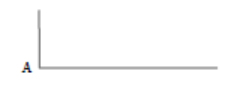
\includegraphics[width=0.5\columnwidth]{figs/16.png}
    \caption{}
    \label{fig:placeholder}
\end{figure}
\begin{multicols}{2}
\begin{enumerate}
    \item does not move horizontally or axially, but moves vertically
    \item does not move axially, but moves both vertically and horizontally
    \item does not move horizontally, vertically or axially
    \item does not move vertically or axially, but moves horizontally
\end{enumerate}
\end{multicols}

% Q17
\item The channel section of uniform thickness 2 mm shown in the figure is subjected to a torque of 10 Nm. If it is made of a material with shear modulus of 25 GPa, the twist per unit length in radians/m is \underline{\hspace{3cm}}
\hfill(GATE AE 2013)

\begin{figure}[H]
    \centering
    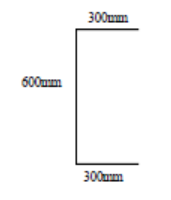
\includegraphics[width=0.35\columnwidth]{figs/17.png}
    \caption{}
    \label{fig:placeholder}
\end{figure}

% Q18
\item The stiffened cross-section of a long slender uniform structural member is idealized as shown in the figure below. The lumped areas at A, B, C and D have equal cross-sectional area of 3 cm$^2$. The webs AB, BC, CD and DA are each 5 mm thick. The structural member is subjected to a twisting moment of 10 kNm. The magnitudes of the shear flow in the webs, $q_{AB}, q_{BC}, q_{CD}$ and $q_{DA}$ in kN/m are, respectively \underline{\hspace{3cm}}
\hfill(GATE AE 2013)

\begin{figure}
    \centering
    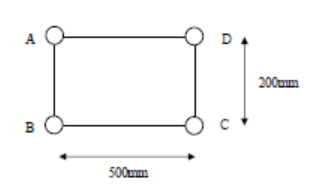
\includegraphics[width=0.5\columnwidth]{figs/18.png}
    \caption{Enter Caption}
    \label{fig:placeholder}
\end{figure}

\begin{multicols}{2}
\begin{enumerate}
    \item 20, 20, 20, 20  
    \item 0, 0, 50, 50  
    \item 40, 40, 0, 0  
    \item 50, 50, 50, 50  
\end{enumerate}
\end{multicols}

% Q19
\item Consider two engines P and Q. In P, the high pressure turbine blades are cooled with a bleed of 5\% from the compressor after the compression process and in Q the turbine blades are not cooled. Comparing engine P with engine Q, which one of the following is NOT TRUE? 
\hfill(GATE AE 2013)

\begin{enumerate}
    \item Turbine inlet temperature is higher for engine P  
    \item Specific thrust is higher for engine P  
    \item Compressor work is the same for both P and Q  
    \item Fuel flow rate is lower for engine P  
\end{enumerate}

% Q20
\item The mass flow rate of air through an aircraft engine is 10 kg/s. The compressor outlet temperature is 400 K and the turbine inlet temperature is 1800 K. The heating value of the fuel is 42 MJ/kg and the specific heat at constant pressure is 1 kJ/kg-K. The mass flow rate of the fuel in kg/s is approximately \underline{\hspace{3cm}}
\hfill(GATE AE 2013)

% Q21
\item For a given inlet condition, if the turbine inlet temperature is fixed, what value of compressor efficiency given below leads to the lowest amount of fuel added in the combustor of a gas turbine engine? 
\hfill(GATE AE 2013)

\begin{multicols}{2}
\begin{enumerate}
    \item 1  
    \item 0.95  
    \item 0.85  
    \item 0.8  
\end{enumerate}
\end{multicols}

% Q22
\item A gas turbine engine is mounted on an aircraft which can attain a maximum altitude of 11 km from sea level. The combustor volume of this engine is decided based on conditions at \underline{\hspace{3cm}}
\hfill(GATE AE 2013)

\begin{multicols}{2}
\begin{enumerate}
    \item sea level  
    \item 8 km altitude  
    \item 5.5 km altitude  
    \item 11 km altitude  
\end{enumerate}
\end{multicols}

% Q23
\item Consider the low earth orbit (LEO) and the geo synchronous orbit (GSO). Then 
\hfill(GATE AE 2013)

\begin{enumerate}
    \item $\Delta V$ requirement for launch to LEO is greater than that for GSO, and altitude of LEO is lower than that of GSO  
    \item $\Delta V$ requirement for launch to LEO is lower than that for GSO, and altitude of LEO is lower than that of GSO  
    \item $\Delta V$ requirement for launch to LEO is greater than that for GSO, and altitude of LEO is greater than that of GSO  
    \item $\Delta V$ requirement for launch to LEO is lower than that for GSO, and altitude of LEO is greater than that of GSO  
\end{enumerate}

% Q24
\item Which one of the following shows the CORRECT variation of stagnation temperature along the axis of an ideal ram jet engine? 
\hfill(GATE AE 2013)

\begin{multicols}{2}
\begin{enumerate}
    \item  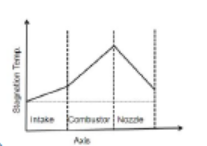
\includegraphics[width=0.5\columnwidth]{figs/A.png}
  
    \item 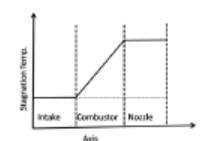
\includegraphics[width=0.5\columnwidth]{figs/B.png}
    
    \item 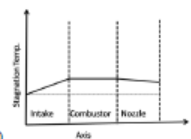
\includegraphics[width=0.5\columnwidth]{figs/C.png}
    
    \item 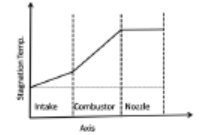
\includegraphics[width=0.5\columnwidth]{figs/D.png}
\end{enumerate}
\end{multicols}

% Q25
\item A rocket motor has a chamber pressure of 100 bar and chamber temperature of 3000 K. The ambient pressure is 1 bar. Assume that the specific heat at constant pressure is 1 kJ/kg-K. Also assume that the flow in the nozzle is isentropic and optimally expanded. The exit static temperature in K is \underline{\hspace{3cm}}
\hfill(GATE AE 2013)

\begin{multicols}{2}
\begin{enumerate}
    \item 805  
    \item 845  
    \item 905  
    \item 945  
\end{enumerate}
\end{multicols}


% Q26
\item Let 
\[
I = \iint_{S} (y^2 \hat{i} + x^2 \hat{j} + x^2 y \hat{k})(x\hat{i} + y\hat{j} + z\hat{k}) \, dS ,
\]
where $S$ denotes the surface of the sphere of unit radius centered at the origin. Here $\hat{i}, \hat{j}, \hat{k}$ denote three orthogonal unit vectors. The value of $I$ is \underline{\hspace{3cm}}
\hfill(GATE AE 2013)

\begin{multicols}{2}
\begin{enumerate}
    \item $0$  
    \item $\dfrac{4\pi}{3}$  
    \item $\dfrac{8\pi}{3}$  
    \item $4\pi$  
\end{enumerate}
\end{multicols}

% Q27
\item Given that the Laplace transform, 
\[
\mathcal{L}(e^{at}) = \frac{1}{s-a},
\] 
then 
\[
\mathcal{L}(3e^{5t} \sinh 5t) =
\]
\hfill(GATE AE 2013)

\begin{multicols}{2}
\begin{enumerate}
    \item $\dfrac{3s}{s^2 - 10s}$  
    \item $\dfrac{15}{s^2 - 10s}$  
    \item $\dfrac{3s}{s^2 + 10s}$  
    \item $\dfrac{15}{s^2 + 10s}$  
\end{enumerate}
\end{multicols}

% Q28
\item Values of $a, b, c$ which render the matrix
\[
Q = \myvec{ \dfrac{1}{\sqrt{3}} & \dfrac{1}{\sqrt{2}} & a \\[6pt]
           \dfrac{1}{\sqrt{3}} & 0 & b \\[6pt]
           \dfrac{1}{\sqrt{3}} & \dfrac{1}{\sqrt{2}} & c }
\]
orthonormal are, respectively
\hfill(GATE AE 2013)

\begin{multicols}{2}
\begin{enumerate}
    \item $\dfrac{1}{\sqrt{2}}, \dfrac{1}{\sqrt{2}}, 0$  
    \item $\dfrac{1}{\sqrt{6}}, -\dfrac{2}{\sqrt{6}}, \dfrac{1}{\sqrt{6}}$  
    \item $\dfrac{1}{\sqrt{3}}, \dfrac{1}{\sqrt{3}}, \dfrac{1}{\sqrt{3}}$  
    \item $-\dfrac{1}{\sqrt{6}}, \dfrac{2}{\sqrt{6}}, -\dfrac{1}{\sqrt{6}}$  
\end{enumerate}
\end{multicols}

% Q29
\item A function $y(t)$ satisfies the differential equation
\[
\frac{d^2 y}{dt^2} - 2\frac{dy}{dt} + y = 0
\]
and is subject to the initial conditions $y(t=0) = 0$ and $\dfrac{dy}{dt}(t=0) = 1$.  
The value of $y(t=1)$ is \underline{\hspace{3cm}}
\hfill(GATE AE 2013)

\begin{multicols}{2}
\begin{enumerate}
    \item $e$  
    \item $0$  
    \item $1$  
    \item $-1$  
\end{enumerate}
\end{multicols}

% Q30
\item A glider is launched from a 500\,m high hilltop. Following data is available for the glider. Zero lift drag coefficient $C_{D0}=0.02$, aspect ratio $AR=10$ and Oswald efficiency factor $e=0.95$. The maximum range of the glider in km is \underline{\hspace{3cm}} 
\hfill(GATE AE 2013)

% Q31
\item Which one of the following criteria leads to maximum turn rate and minimum radius in a level turn flight? 
\hfill(GATE AE 2013)

\begin{enumerate}
  \item Highest possible load factor and highest possible velocity
  \item Lowest possible load factor and lowest possible velocity
  \item Highest possible load factor and lowest possible velocity
  \item Lowest possible load factor and highest possible velocity
\end{enumerate}

% Q32
\item Consider an airplane with rectangular straight wing at dihedral angle $\Gamma=10^\circ$. Lift curve slope of wing airfoil section (constant over the whole span of the wing) is $c_{\ell\alpha}=5.4/\mathrm{rad}$. The roll stability derivative, $C_{\ell_\beta}$ in per radian is \underline{\hspace{3cm}} 
\hfill(GATE AE 2013)

% Q33
\item Consider one-dimensional isentropic flow at a Mach number of $0.5$. If the area of cross-section of a streamtube increases by $3\%$ somewhere along the flow, the corresponding percentage change in density is \underline{\hspace{3cm}} 
\hfill(GATE AE 2013)

% Q34
\item The potential flow model for a storm is represented by the superposition of a sink and a vortex. The stream function in the $(r,\theta)$ system is
\[
\psi \;=\; -\frac{\Delta}{2\pi}\,r \;+\; \frac{\Gamma}{2\pi}\ln r ,
\]
where $\Delta=-\Gamma=100~\mathrm{m^2/s}$. Assume a constant air density of $1.2~\mathrm{kg/m^3}$. The gauge pressure at a distance of $100$ m from the storm eye is
\hfill(GATE AE 2013)

\begin{multicols}{2}
\begin{enumerate}
  \item $-\infty$
  \item $\dfrac{1.2}{\pi r^{2}}$
  \item $-\dfrac{1.2}{2\pi r^{2}}$
  \item $\dfrac{1.2}{4\pi r^{2}}$
\end{enumerate}
\end{multicols}

% Q35
\item Three identical eagles of wing span $s$ are flying side by side in a straight line with no gap between their wing tips. Assume a single horseshoe vortex model (of equal strength $\Gamma$) for each bird. The net downwash experienced by the middle bird is
\hfill(GATE AE 2013)

\begin{multicols}{2}
\begin{enumerate}
  \item $\dfrac{\Gamma}{\pi s}$
  \item $\dfrac{\Gamma}{2\pi s}$
  \item $\dfrac{2\Gamma}{3\pi s}$
  \item $\dfrac{4\Gamma}{3\pi s}$
\end{enumerate}
\end{multicols}

% Q36
\item Streamline pattern of flow past a cylinder is shown in the figure. The oncoming flow is steady, irrotational and incompressible. The flow is from left to right. Bernoulli's equation \emph{cannot} be applied between the points
\hfill(GATE AE 2013)
\begin{figure}[H]
    \centering
    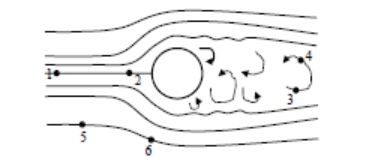
\includegraphics[width=0.5\columnwidth]{figs/36.png}
    \caption{}
    \label{fig:placeholder}
\end{figure}
\begin{multicols}{2}
\begin{enumerate}
  \item 1 and 2
  \item 1 and 5
  \item 3 and 4
  \item 5 and 6
\end{enumerate}
\end{multicols}

% Q37
\item Consider a supersonic stream at a Mach number $M=2$, undergoing a gradual expansion. The stream is turned by an angle of $3^\circ$ due to the expansion. The following data is given:

\begin{center}
\begin{tabular}{|c|c|}

\hline
$M$ & $\nu$ 
(Prandtl--Meyer function) \\
\hline
1.8 & 20.73 \\
1.9 & 23.59 \\
2.0 & 26.38 \\
2.1 & 29.10 \\
2.2 & 31.73 \\
2.3 & 34.28 \\
2.4 & 36.75 \\
\hline
\end{tabular}
\end{center}
\hfill(GATE AE 2013)

\begin{multicols}{2}
\begin{enumerate}
  \item 1.88
  \item 2.00
  \item 2.11
  \item 2.33
\end{enumerate}
\end{multicols}

% Q38
\item The idealized cross-section of a beam is comprised of four identical booms connected by shear webs. The beam is subjected to a bending moment $M$ as shown in the figure. The inclination of the neutral axis to the $y$-axis in degrees is

\hfill(GATE AE 2013)
\begin{figure}[H]
    \centering
    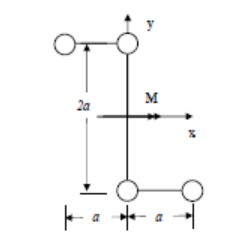
\includegraphics[width=0.35\columnwidth]{figs/38.png}
    \caption{}
    \label{fig:placeholder}
\end{figure}
\begin{multicols}{2}
\begin{enumerate}
  \item 45 CW
  \item 45 CCW
  \item 26.6 CW
  \item 63.4 CCW
\end{enumerate}
\end{multicols}

% Q39
\item A composite circular shaft is comprised of a steel core surrounded by an aluminum annulus, perfectly bonded to each other as shown in the figure. If subjected to a pure torque, which one of the following statements is TRUE?
\hfill(GATE AE 2013)
\begin{figure}[H]
    \centering
    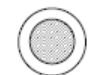
\includegraphics[width=0.35\columnwidth]{figs/39.png}
    \caption{}
    \label{fig:placeholder}
\end{figure}
\begin{enumerate}
  \item Only shear stress is continuous across the steel-aluminum interface
  \item Only shear strain is continuous across the steel-aluminum interface
  \item Both shear stress and shear strain are continuous across the steel-aluminum interface
  \item Both shear stress and shear strain are discontinuous across the steel-aluminum interface
\end{enumerate}

% Q40
\item A horizontal rectangular plate $ABCD$ is hinged at points $A,B$ and $C$, and $BD$ are diagonals of the plate. Downward force $P$ is applied at $D$. The upward reactions $R_A,R_B$ and $R_C$ at points $A,B$ and $C$, respectively, are
\hfill(GATE AE 2013)

\begin{multicols}{2}
\begin{enumerate}
  \item indeterminate
  \item $P,-P,P$
  \item $0,P,0$
  \item $P/3,P/3,P/3$
\end{enumerate}
\end{multicols}

\item In the steel structure (Young's modulus = 200 GPa) shown in the figure, all members have a circular cross-section of radius 10 mm. Column BD is pinned at B and D. The support at A is hinged. The minimum value of load P at which the column BD may buckle in Newtons is approximately \underline{\hspace{2cm}}. 
\begin{figure}[H]
    \centering
    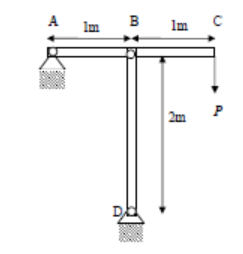
\includegraphics[width=0.5\columnwidth]{figs/41.png}
    \caption{}
    \label{fig:placeholder}
\end{figure}
\hfill(GATE AE 2013)

\item The thin rectangular plate has dimensions L x b x t. It develops a stress field corresponding to an applied bending moment M as shown in the figure. A valid Airy's stress function is

\hfill(GATE AE 2013)

\begin{figure}[H]
    \centering
    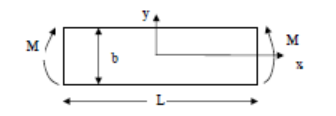
\includegraphics[width=0.5\columnwidth]{figs/42.png}
    \caption{}
    \label{fig:placeholder}
\end{figure}
\begin{multicols}{2}
\begin{enumerate}
\item $\dfrac{2M}{tb^3}x^3$
\item $\dfrac{2M}{tb^3}y^3$
\item $\dfrac{2M}{tb^3}(x^3+y^3)$
\item $\dfrac{2M}{tb^3}y^4$
\end{enumerate}
\end{multicols}

\item A cantilever beam of negligible mass is 0.6 m long. It has a rectangular cross-section of width 8 mm and thickness 6 mm and carries a tip mass of 1.4 kg. If the natural frequency of this system is 10 rad/s, Young's modulus of the material of the beam in GPa is \underline{\hspace{2cm}}. \hfill(GATE AE 2013)

\item A simply supported beam with overhang is loaded by uniformly distributed load of intensity $q$ as shown in the figure. The bending moment at the mid-point of AB is \hfill(GATE AE 2013)
\begin{multicols}{2}
\begin{enumerate}
\item $\dfrac{qL^2}{16}$ sagging
\item $\dfrac{qL^2}{16}$ hogging
\item $\dfrac{3qL^2}{16}$ hogging
\item $\dfrac{3qL^2}{16}$ sagging
\end{enumerate}
\end{multicols}

\item Thrust of liquid oxygen-liquid hydrogen rocket engine is 300 kN. The O/F ratio used is 5. If the fuel mass flow rate is 12.5 kg/s, the specific impulse of the rocket motor in Ns/kg is

\hfill(GATE AE 2013)
\begin{multicols}{2}
\begin{enumerate}
\item 3800
\item 4000
\item 4200
\item 4400
\end{enumerate}
\end{multicols}

\item In a 50\% reaction axial compressor stage, the local blade velocity is 300 m/s and the axial component of velocity is 100 m/s. If the absolute inlet flow angle $\alpha_1 = 45^\circ$, the work per unit mass done on the fluid by the stage in kJ/kg is \hfill(GATE AE 2013)
\begin{multicols}{2}
\begin{enumerate}
\item 30
\item 40
\item 50
\item 60
\end{enumerate}
\end{multicols}

\item Consider two rockets P and Q fired vertically up with identical specific impulse and a payload of 2 kg. Rocket P has 2 identical stages, and each stage has 200 kg of propellant and 20 kg of structural weight. Rocket Q has a single stage with 400 kg of propellant and 40 kg of structural weight. Neglecting drag and gravity effects, the ratio of the change in velocity of P to that attained by Q is 

\hfill(GATE AE 2013)
\begin{multicols}{2}
\begin{enumerate}
\item 1.13
\item 1.23
\item 1.33
\item 1.43
\end{enumerate}
\end{multicols}
\textbf{Common Data for Questions 48 and 49:}

Data for an airplane are given as follows: weight $W=30$ kN, thrust available at sea-level $T_a=4000$ N, wing planform area $S=30$ m$^2$, maximum lift coefficient $C_{L_{max}}=1.4$, and drag coefficient $C_D=0.015+0.024C_L^2$. Assume air density at sea-level $\rho_\infty=1.22$ kg/m$^3$. 
\item Stall speed of the airplane in m/s is \hfill(GATE AE 2013)
\begin{multicols}{2}
\begin{enumerate}
\item 17.36
\item 34.22
\item 45.52
\item 119.46
\end{enumerate}
\end{multicols}

\item Minimum and maximum speeds of the airplane in level flight condition at sea-level in m/s are respectively 

\hfill(GATE AE 2013)
\begin{multicols}{2}
\begin{enumerate}
\item 17.36 and 180
\item 17.36 and 34.22
\item 34.22 and 119.46
\item 17.36 and 119.46
\end{enumerate}
\end{multicols}
\textbf{Common Data for Questions 50 and 51:} 

An aircraft is flying at Mach number $M = 1.5$, where the ambient temperature is $250 \;K$. The stagnation temperature of gases at the entry to the nozzle is $800 \;K$. The nozzle is choked and always under expanded. Assume the molecular weight of the exhaust gases to be $29$, the ratio of specific heats to be $1.4$ and the universal gas constant is $8314 \; J/kmol\cdot K$. 


\item For which one of the nozzle exit Mach numbers given below is the propulsive efficiency highest? 

\hfill(GATE AE 2013)
\begin{multicols}{2}
\begin{enumerate}
\item 1
\item 1.5
\item 2
\item 2.5
\end{enumerate}
\end{multicols}

\item For which one of the nozzle exit Mach numbers given below is the thrust highest? 

\hfill(GATE AE 2013)
\begin{multicols}{2}
\begin{enumerate}
\item 1
\item 1.5
\item 2
\item 2.5
\end{enumerate}
\end{multicols}



\textbf{Statement for Linked Answer Questions 52 and 53:}

Circulation theory of lift is assumed for a thin symmetric airfoil at an angle of attack $\alpha$. Free stream velocity is $U$.


\item If the circulation at the quarter chord ($c/4$) of the airfoil is $\Gamma_1$, the normal velocity is zero at

\hfill(GATE AE 2013)
\begin{multicols}{2}
\begin{enumerate}
\item $c/4$
\item $c/2$
\item $3c/4$
\item all points on the chord
\end{enumerate}
\end{multicols}

\item A second identical airfoil is placed behind the first one at a distance of $c/2$ from the trailing edge of the first. The second airfoil has an unknown circulation $\Gamma_2$ placed at its quarter chord. The normal velocity becomes zero at the same chord-wise locations of the respective airfoils as in the previous question. The values of $\Gamma_1$ and $\Gamma_2$ are respectively \hfill(GATE AE 2013)
\begin{multicols}{2}
\begin{enumerate}
\item $\dfrac{4}{3}\pi cU \alpha, \;\; \dfrac{2}{3}\pi cU \alpha$
\item $\dfrac{2}{3}\pi cU \alpha, \;\; \dfrac{2}{3}\pi cU \alpha$
\item $\dfrac{2}{3}\pi cU \alpha, \;\; \dfrac{1}{3}\pi cU \alpha$
\item $\dfrac{4}{3}\pi cU \alpha, \;\; \dfrac{4}{3}\pi cU \alpha$
\end{enumerate}
\end{multicols}

\textbf{Statement for Linked Answer Questions 54 and 55:}

A wing-body alone configuration airplane with a wing loading of $\dfrac{W}{S} = 1000 \, N/m^2$ is flying in cruise condition at a speed $V = 90 \, m/s$ at sea-level (air density at sea-level, $\rho_\infty = 1.22 \, kg/m^3$). The zero lift pitching moment coefficient of the airplane is $C_{m0} = -0.06$ and the location of airplane aerodynamic center from the wing leading edge is $X_{ac} = 0.25c$. Here $c$ is the chord length.

\item The airplane trim lift coefficient $C_{L_{trim}}$ is 

\hfill(GATE AE 2013)
\begin{multicols}{2}
\begin{enumerate}
\item 0.502
\item 0.402
\item 0.302
\item 0.202
\end{enumerate}
\end{multicols}

\item Distance of center of gravity of the aircraft $(X_{cg})$ from the wing leading edge is 

\hfill(GATE AE 2013)
\begin{multicols}{2}
\begin{enumerate}
\item 0.447c
\item -0.547c
\item 0.547c
\item -0.25c
\end{enumerate}
\end{multicols}
\begin{center}
\textbf{General Aptitude (GA) Questions}     
\end{center}


\textbf{Q.56 -- Q.60 carry one mark each.}
\item If $3 \leq X \leq 5$ and $8 \leq Y \leq 11$ then which of the following options is TRUE? 

\hfill(GATE AE 2013)
\begin{multicols}{2}
\begin{enumerate}
\item $\dfrac{3}{5} \leq \dfrac{X}{Y} \leq \dfrac{8}{5}$
\item $\dfrac{3}{11} \leq \dfrac{X}{Y} \leq \dfrac{5}{8}$
\item $\dfrac{3}{11} \leq \dfrac{X}{Y} \leq \dfrac{8}{5}$
\item $\dfrac{3}{5} \leq \dfrac{X}{Y} \leq \dfrac{8}{11}$
\end{enumerate}
\end{multicols}

\item The Headmaster \underline{\hspace{2cm}} to speak to you. 

Which of the following options is incorrect to complete the above sentence? 
\hfill(GATE AE 2013)
\begin{multicols}{2}
\begin{enumerate}
\item is wanting
\item wants
\item want
\item was wanting
\end{enumerate}
\end{multicols}

\item Mahatma Gandhi was known for his humility as

\hfill(GATE AE 2013)
\begin{multicols}{2}
\begin{enumerate}
\item he played an important role in humiliating exit of British from India.
\item he worked for humanitarian causes.
\item he displayed modesty in his interactions.
\item he was a fine human being.
\end{enumerate}
\end{multicols}

\item \underline{All engineering students}(I)\quad \underline{should learn mechanics}(II) \quad \underline{mathematics and}(III) \quad \underline{ how to do computation.}(IV)

Which of the above underlined parts of the sentence is not appropriate? \hfill(GATE AE 2013)
\begin{multicols}{2}
\begin{enumerate}
\item I
\item II
\item III
\item IV
\end{enumerate}
\end{multicols}

\item Select the pair that best expresses a relationship similar to that expressed in the pair: 
\hspace{1cm} water : pipe ::

\hfill(GATE AE 2013)
\begin{multicols}{2}
\begin{enumerate}
\item cart : road
\item electricity : wire
\item sea : beach
\item music : instrument
\end{enumerate}
\end{multicols}

\textbf{Q.61 to Q.65 carry two marks each.}

\item Velocity of an object fired directly in upward direction is given by $V = 80 - 32t$, where $t$ (time) is in seconds. When will the velocity be between 32 m/sec and 64 m/sec? \hfill(GATE AE 2013)
\begin{multicols}{2}
\begin{enumerate}
\item (2, 3/2)
\item (1/2, 1)
\item (1/2, 3/2)
\item (1, 3)
\end{enumerate}
\end{multicols}

\item In a factory, two machines M1 and M2 manufacture 60\% and 40\% of the autocomponents respectively. Out of the total production, 2\% of M1 and 3\% of M2 are found to be defective. If a randomly drawn autocomponent from the combined lot is found defective, what is the probability that it was manufactured by M2? \hfill(GATE AE 2013)
\begin{multicols}{2}
\begin{enumerate}
\item 0.35
\item 0.45
\item 0.50
\item 0.40
\end{enumerate}
\end{multicols}

\item Following table gives data on tourists from different countries visiting India in the year 2011. 
\begin{center}
\begin{tabular}{|c|c|}
\hline
\textbf{Country} & \textbf{Number of Tourists} \\
\hline
USA & 2000 \\
England & 3500 \\
Germany & 1200 \\
Italy & 1100 \\
Japan & 2400 \\
Australia & 2300 \\
France & 1000 \\
\hline
\end{tabular}
\end{center}

Which two countries contributed to one third of the total number of tourists who visited India in 2011? \hfill(GATE AE 2013)

\begin{multicols}{2}
\begin{enumerate}
\item USA and Japan
\item USA and Australia
\item England and France
\item Japan and Australia
\end{enumerate}
\end{multicols}


\item If $\lvert -2X + 9 \rvert = 3$ then the possible value of $\lvert -X \rvert - X^2$ would be: 

\hfill(GATE AE 2013)
\begin{multicols}{2}
\begin{enumerate}
\item 30
\item -30
\item -42
\item 42
\end{enumerate}
\end{multicols}

\item All professors are researchers. 

Some scientists are professors. 

Which of the given conclusions is logically valid and is inferred from the above arguments: 

\hfill(GATE AE 2013)

\begin{multicols}{2}
\begin{enumerate}
\item All scientists are researchers
\item All professors are scientists
\item Some researchers are scientists
\item No conclusion follows
\end{enumerate}
\end{multicols}

\begin{center}
\textbf{END OF THE QUESTION PAPER}
\end{center}

\end{enumerate}
\end{flushleft}
\end{document}






